% !TeX root = ../thesis_main.tex

% ---------------------------------------------------
% ----- Chapters of the template
% ----- for Bachelor-, Master thesis and class papers
% ---------------------------------------------------
%  Created by C. Müller-Birn on 2012-08-17, CC-BY-SA 3.0.
%  Freie Universität Berlin, Institute of Computer Science, Human Centered Computing. 
%
% TODO remove 2 - to use auto numbering
\chapter{Prototyping}
\label{chap:prototyping} 

After collecting the inital user feedback, I started drawing minimal digital ''paper'' prototypes using Figma to gather vizualizations of the proposed UI layouts.
Two ideas emerged from the interviews: a (file-)editor-centric layout and a preview-centric layout.
\section{Editor centric vs preview centric layout}
The editor-centric layout is inspired by modern text editors / IDEs like VS Code (\url{https://code.visualstudio.com/}), which was mentioned as reference during the interviews multiple times.
There, the central pane is the editor for the currently open file, while on the sides additional panes for file management, preview and more can be shown.
The familarity, especially to developers who are used to IDE layouts, could help new users adopt patterns to work with the UI they use in other tools as well.
\\\\
The idea for a preview-centric layout was inspired by popular generic website builders like \url{https://wix.com} or \url{https://wordpress.com}, where the user
can see the page in an interactive mode, move, configure or place elements, and then has on the side additional panels like one with information \& options about the
currently selected element.
There are also framework-agnostic tools like \url{https://vwo.com/why-us/technology/visual-editor/}, but they either focused more on only editing the style and not the structure of the page or were not
compatible with the Experience's framework and data fromat. 
\\
Ultimately our choice fell to the editor centric layout, the following are some of the reasons for it over the preview-centric one:
\begin{itemize}
  \item The configuration structure of the Experience framework was not built with preview-based editing in mind. A lot of functionality is hidden inside the components and invisible for the user,
  often components only appear under specific conditions that are not easily reproducable in the editor environment. Thus, editing in a preview-centric mode could in many situations
  lead to more confusion by the editors than speed the process up. As the configuration schemata are mostly fixed and I can't prevent 
  \item After evaluation of some avaialble libraries and examples, we concluded that building a reliable and usable preview-centric editor is more complicated, and even without the time restricition of my bachelor thesis, I proposed to not go this way,
  as it was unclear if it even could result in a viable product in reasonable time. For editor-centric UIs, many thirdparty libraries exist, that can be integrated into the UI.
  Some relevant are Monaco Editor (the VS Code Open source text editor part) for editing generic web related files like CSS and JS with automatic syntax highlighting and error detection, and an JSON Editor for work with json configs where we could provide a schema.
  \item The userbase consists mostly of tech-affine people who are used to layouts of IDEs, and the old tool also had a similar editor centric layout.
  As Jakob's Law of the Internet User Experience states (cf. \cite{Nielsen:2000} and \cite[p. 2]{LawsOfUX:2020ys}), the user's understanding of a website is directly tied to his/hers mental model of that system.
  Introducing a unconventional workflow comes with the danger that the user gets confused, makes mistakes or in the worst case doesn't like working with the tool anymore.

\end{itemize}

\begin{figure}[h]
  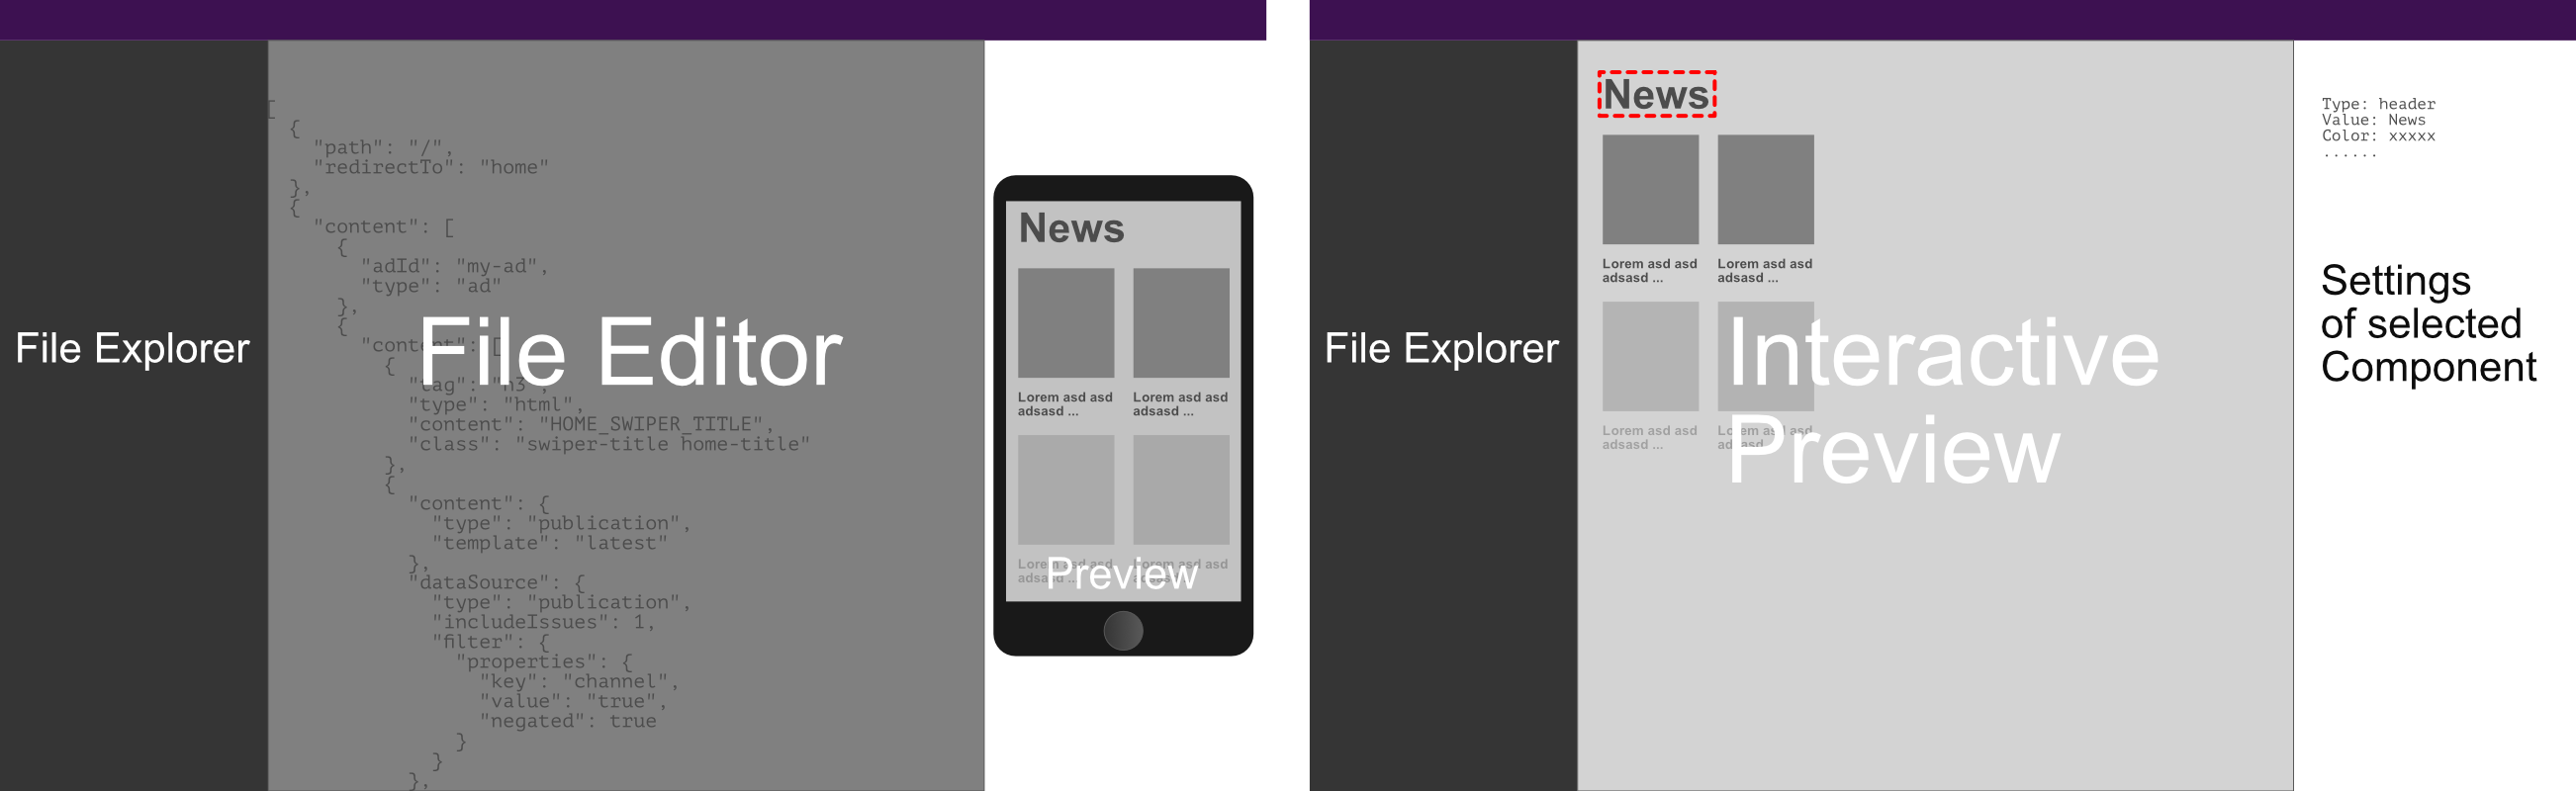
\includegraphics[width=\textwidth]{pics/editor_centric_vs_preview_centric.png}
  \caption{Mockups: Editor centric vs preview centric editor layout}
\end{figure}

